    \subsection[Approx]{Aprrossimazione}
        
        \begin{frame}{Gestione evoluzione}
            Funzione sistema::evo() - loop sul tempo
            \begin{itemize}
                \item[$\Rightarrow$] Funzione sistema::evodt() - loop sui corpi
                \begin{itemize}
                    \item[$\Rightarrow$] Funzione corpo::edolvidt() - aggiornamento posizione/velocità e raccolta dati per ogni corpo
                    \begin{itemize}
                        \item[$\Rightarrow$] Funzione corpo::muovi() - scelta metodo di approssimazione
                    \end{itemize}
                \end{itemize}
            \end{itemize}    

            \begin{exampleblock}{$N>2 \Rightarrow$ Soluzione approssimata tramite metodi iterativi discreti:}
                \begin{enumerate}
                    \item Metodo di Eulero - approssimazione lineare
                \end{enumerate}
                \begin{equation}
                \left\{ 
                \begin{array}{l}
                    \vec{a_i}(t)=f_{GravUniv}(\vec{x_i}(t)) \\
                    \vec{v_i}(t+\Delta t)=\vec{v_i}(t)+\vec{a_i}\Delta t \\
                    \vec{x_i}(t+\Delta t)=\vec{x_i}(t)+\vec{v_i}(t+\Delta t)\Delta t
                \end{array}
                \right.
                \end{equation}
            \end{exampleblock}
        \end{frame}

        \begin{frame}{Gestione evoluzione}
            Funzione sistema::evo() - loop sul tempo
            \begin{itemize}
                \item[$\Rightarrow$] Funzione sistema::evodt() - loop sui corpi
                \begin{itemize}
                    \item[$\Rightarrow$] Funzione corpo::edolvidt() - aggiornamento posizione/velocità e raccolta dati per ogni corpo
                    \begin{itemize}
                        \item[$\Rightarrow$] Funzione corpo::muovi() - scelta metodo di approssimazione
                    \end{itemize}
                \end{itemize}
            \end{itemize}    

            \begin{exampleblock}{$N>2 \Rightarrow$ Soluzione approssimata tramite metodi iterativi discreti:}
                \begin{enumerate}
                    \item Metodo di Eulero - approssimazione lineare
                    \item Runge-Kutta $2^{nd}$ order - Eulero modificato
                \end{enumerate}
                \begin{equation}
                \left\{ 
                \begin{array}{l}
                    \vec{a_i^1}(t)=f_{GravUniv}(\vec{x_i}(t)) \\
                    \vec{x'}(t+\Delta t)=\vec{x_i}(t)+\vec{v_i}(t)\Delta t \\
                    \vec{a_i^2}(t)=f_{GravUniv}(\vec{x'}(t)+\Delta t) \\
                    \vec{v_i}(t+\Delta t)=\vec{v_i}(t)+\frac{\vec{a_i^1}+\vec{a_i^2}(t)}{2}\Delta t \\
                    \vec{x_i}(t+\Delta t)=\vec{x_i}(t)+\frac{\vec{v_i}(t)+\vec{v_i}(t+\Delta t)}{2}\Delta t
                \end{array}
                \right.
                \end{equation}
            \end{exampleblock}
        \end{frame}

        \begin{frame}{deltaT=3600s}
            \begin{columns}
                \column{.4\textwidth}
                \centering
                %\caption{Momento angolare del sistema dopo 2 anni nei due metodi descritti}            
                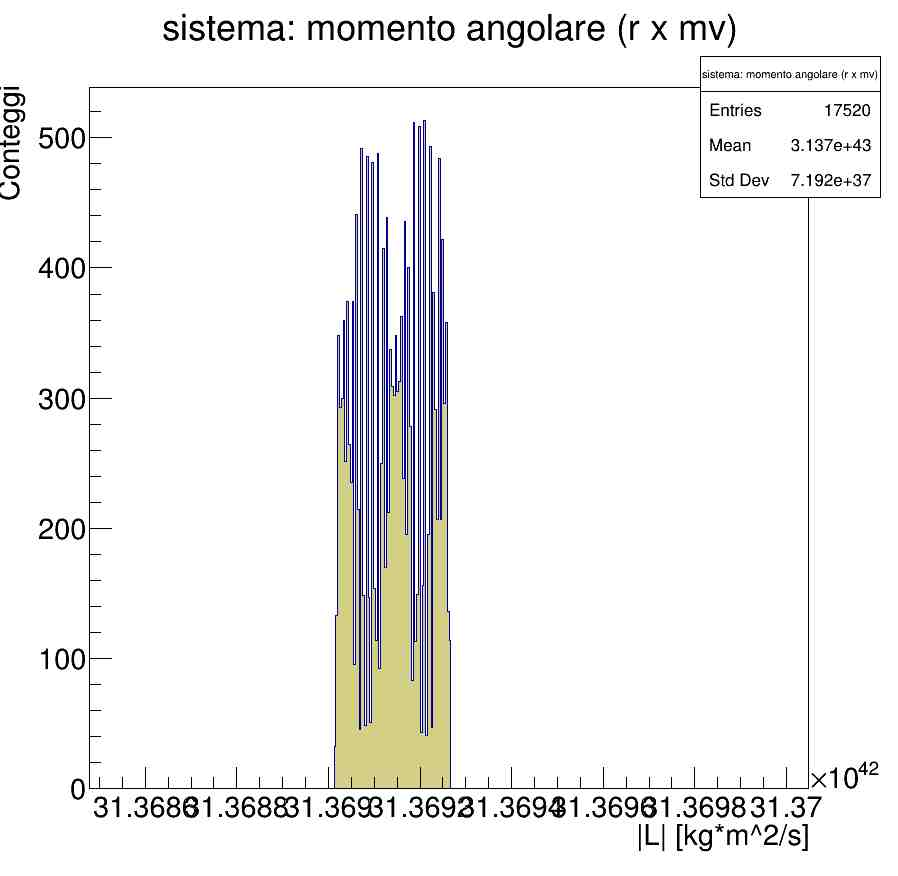
\includegraphics[width=4cm,height=4cm]{2_approx/L_2_0.jpg}\\
                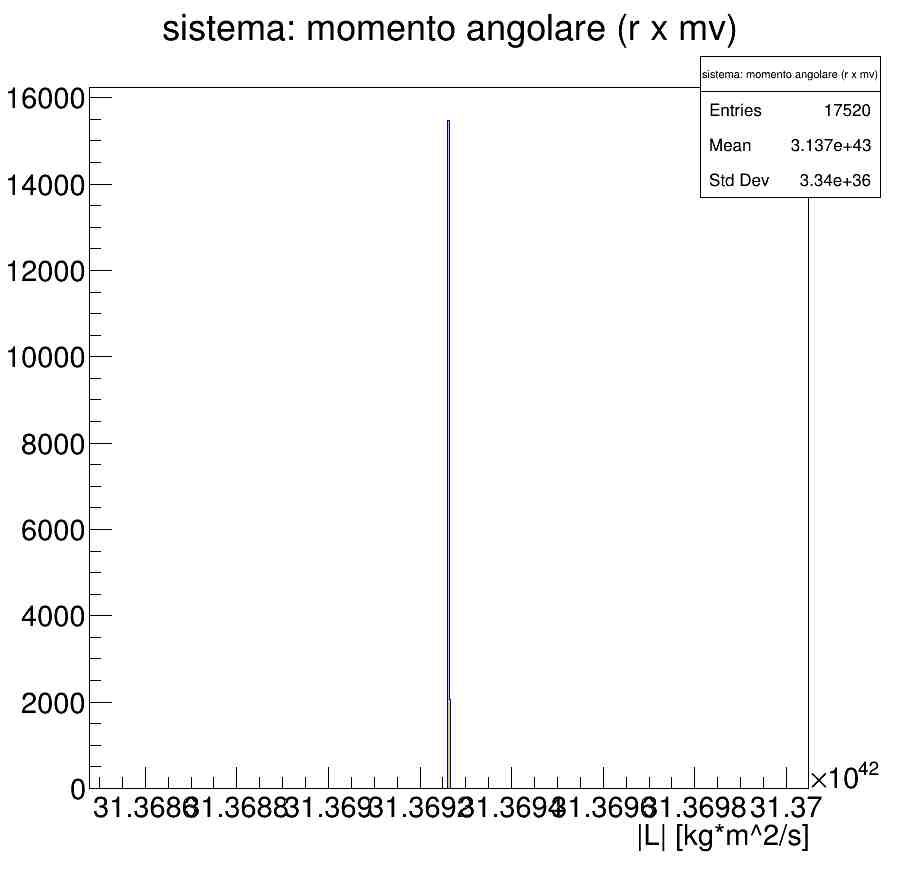
\includegraphics[width=4cm,height=3.5cm]{2_approx/L1_2.jpg}
                \label{cfr::L1}
                \column{.2\textwidth}
                \centering
                Metodo di Eulero\\
                \vspace{2cm}
                Eulero modificato
                \column{.4\textwidth}
                \centering
                %\caption{Orbita terrestre dopo 5 anni nei due metodi descritti}            
                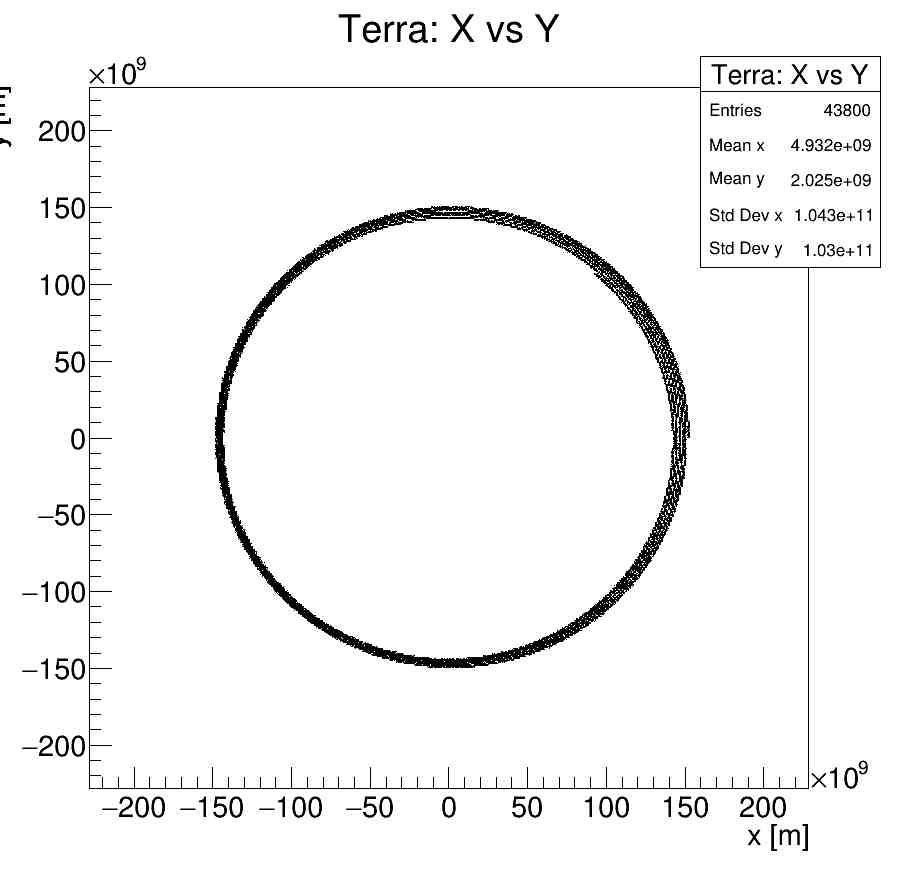
\includegraphics[width=3.75cm,height=3.75cm]{2_approx/terraxy_0_5.jpg}\\
                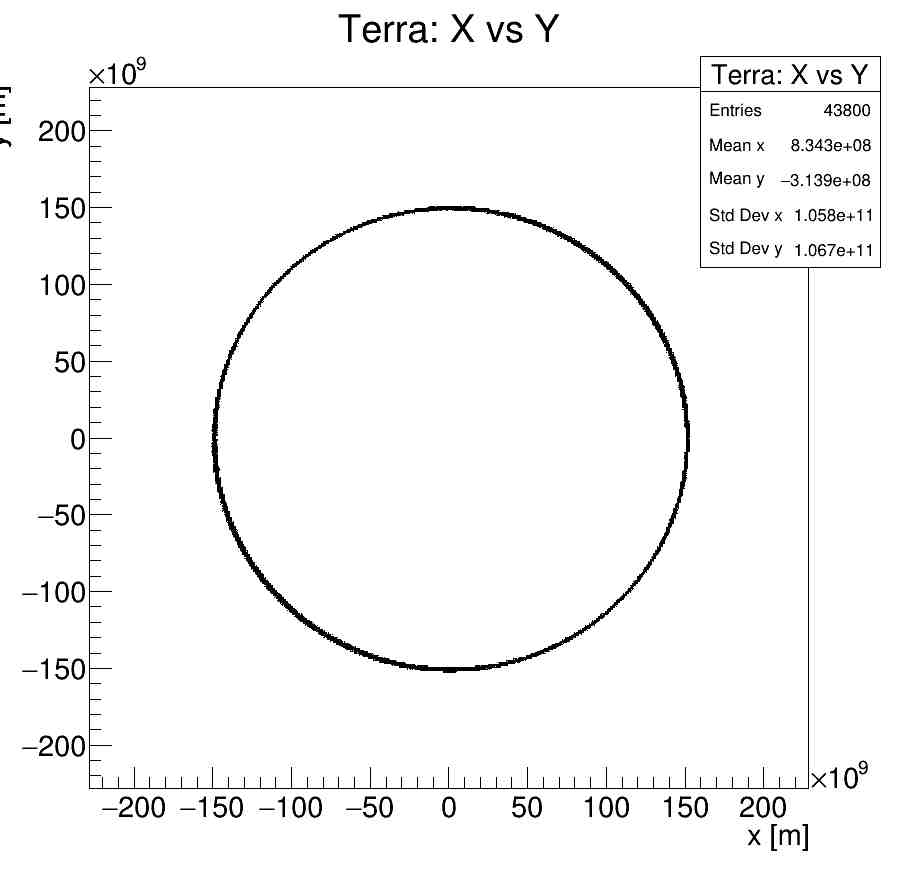
\includegraphics[width=3.75cm,height=3.75cm]{2_approx/terraxy_1_5.jpg}
                \label{cfr::xy1}
            \end{columns}
        \end{frame}
        
        \begin{frame}{deltaT=60s}
            \begin{columns}
                \column{.4\textwidth}
                    \centering
                    %\caption{Momento angolare del sistema dopo 100 anni nei due metodi descritti}            
                    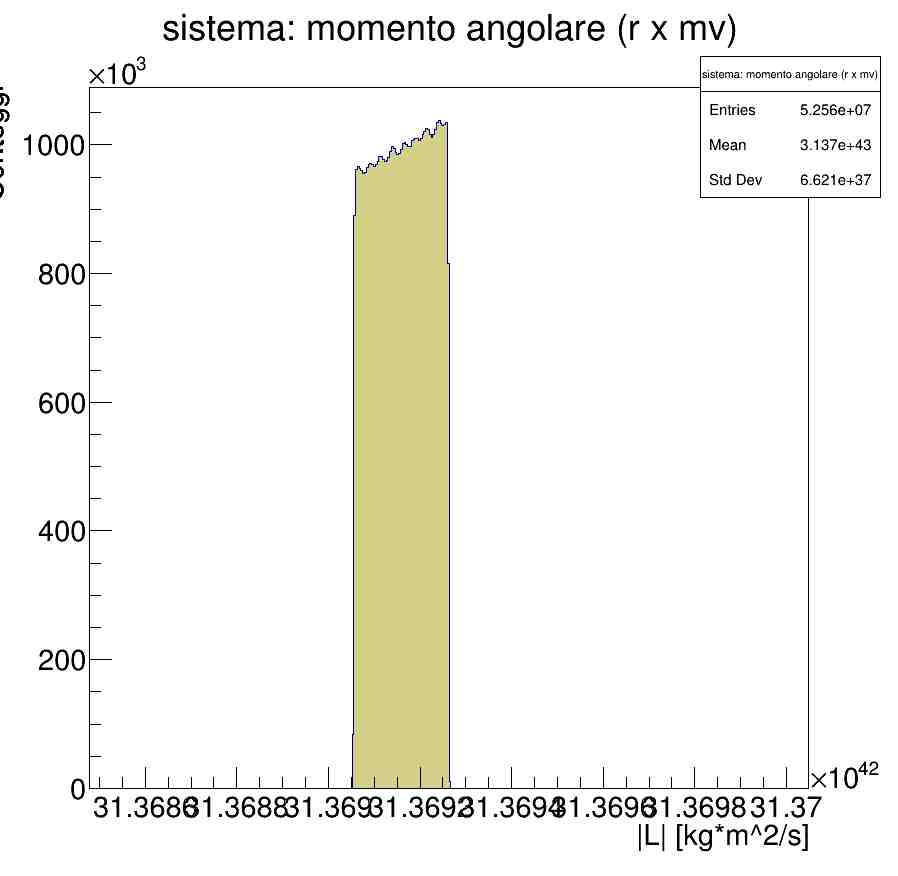
\includegraphics[width=4cm,height=4cm]{2_approx/L0_100.jpg}\\
                    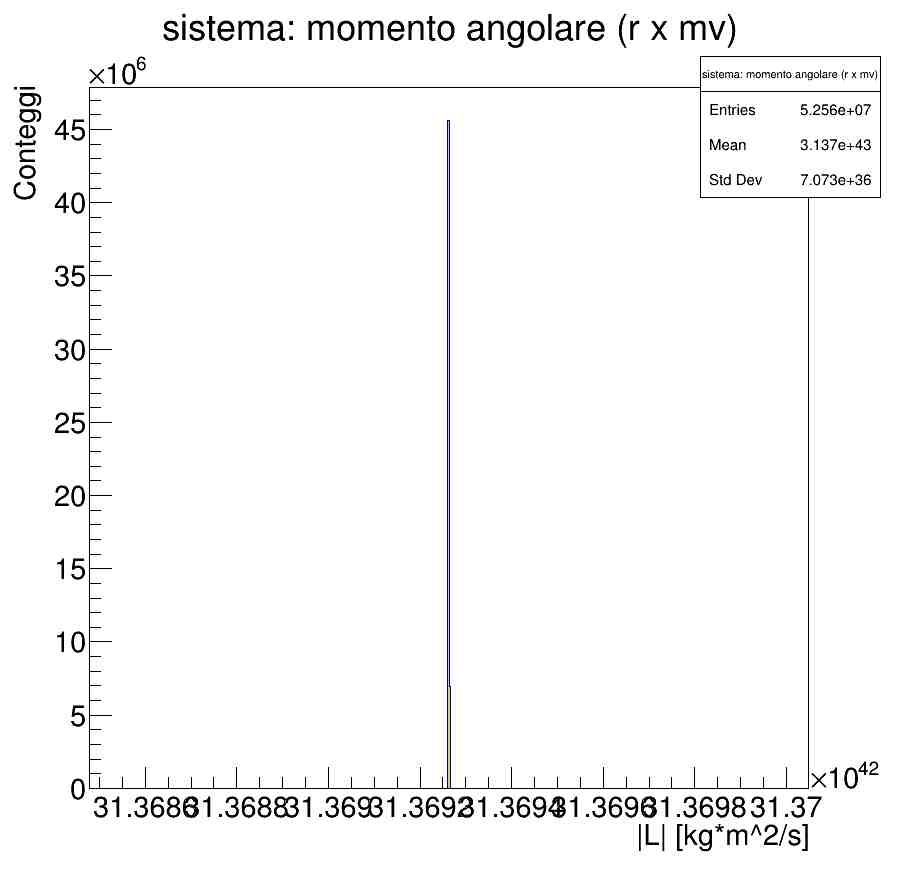
\includegraphics[width=4cm,height=3.5cm]{2_approx/L100_1.jpg}
                    \label{cfr::L2}
                \column{.2\textwidth}
                    \centering
                    Metodo di Eulero\\
                    \vspace{2cm}
                    Eulero modificato
                \column{.4\textwidth}
                    \centering
                    %\caption{Orbita terrestre dopo 100 anni nei due metodi descritti}            
                    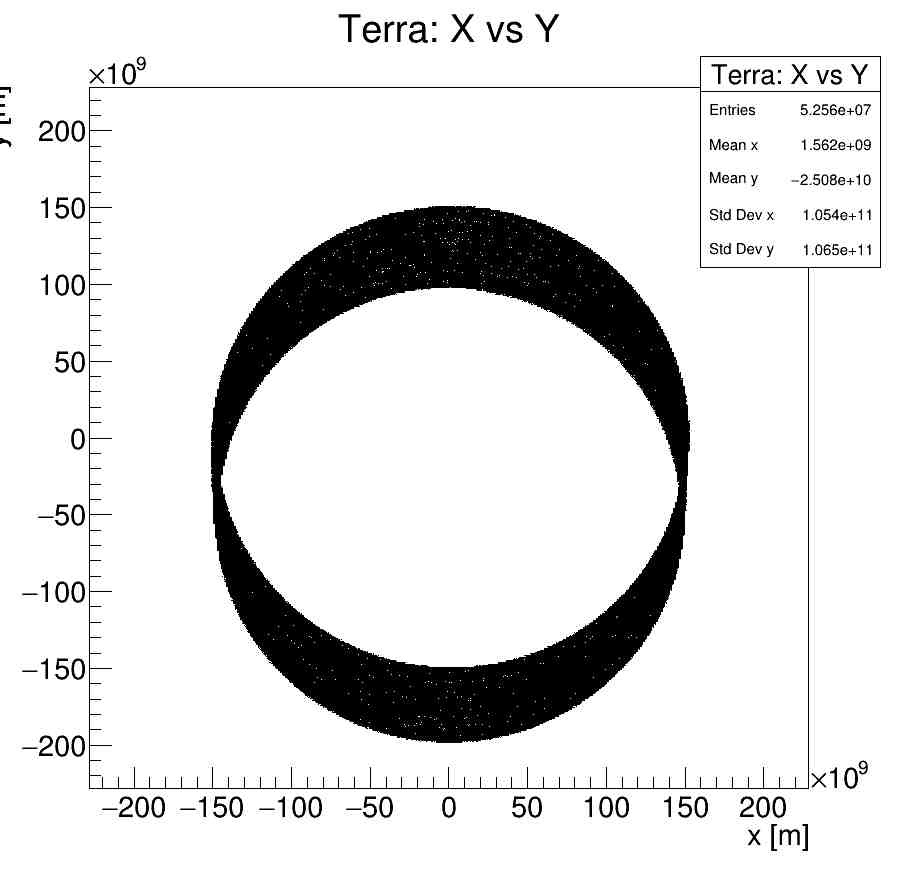
\includegraphics[width=3.75cm,height=3.75cm]{2_approx/terraxy_100_0.jpg}\\
                    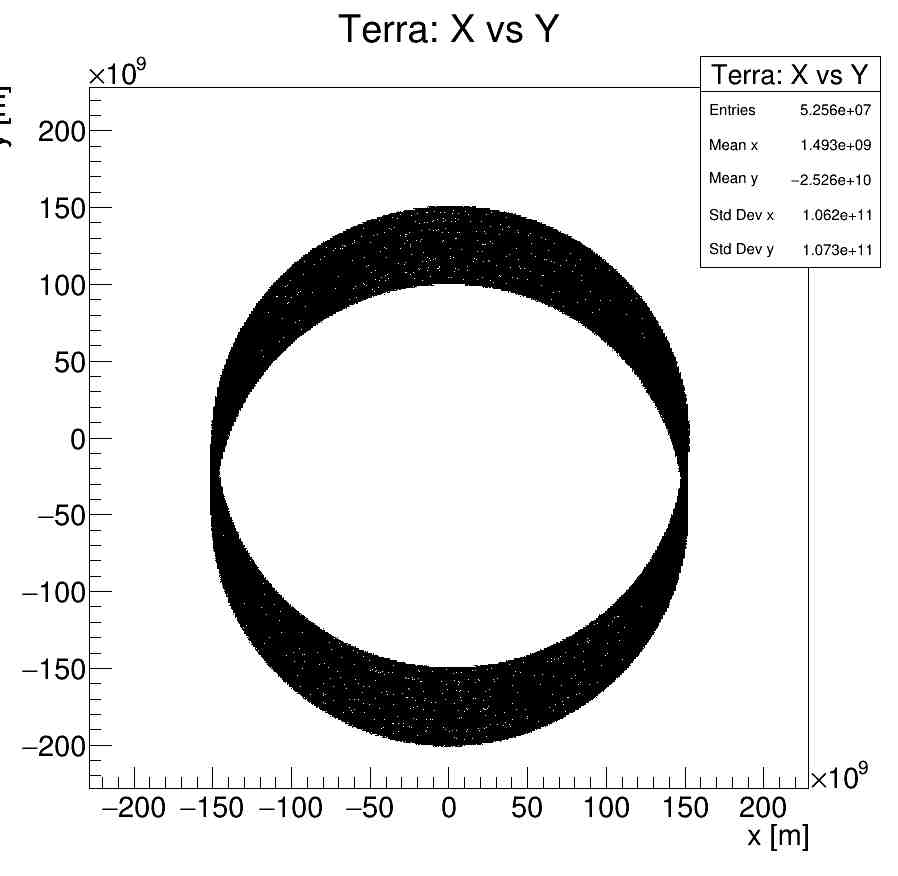
\includegraphics[width=3.75cm,height=3.75cm]{2_approx/terraxy_100__60_1.jpg}
                    \label{cfr::xy2}
            \end{columns}
        \end{frame}

        \begin{frame}{Altri Algoritmi}
            \begin{exampleblock}{$N>2 \Rightarrow$ Soluzione approssimata tramite metodi iterativi discreti:}
                \begin{enumerate}
                    \item Metodo di Eulero - approssimazione lineare
                    \item Runge-Kutta $2^{nd}$ order - Eulero modificato - limite 2000 anni
                    \item Runge-Kutta $2^{nd}$ order - altra versione
                    \item Velocity Verlet - sempre approssimazione del secondo ordine
                    \item Runge-Kutta $4^{th}$ - drifta subito ....
                    \item Yoshida $4^{th}$ order - algoritmo del quarto ordine - ma limiti come per velocity verlet ...
                \end{enumerate}
            \end{exampleblock}
            \begin{figure}
                \centering
                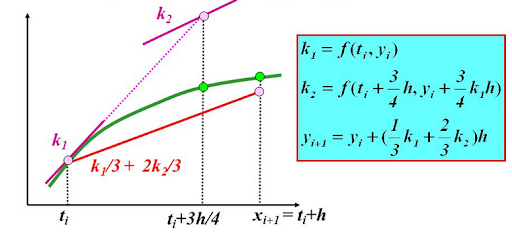
\includegraphics[width=0.5\linewidth]{2_approx/kutta.png}
                %\caption{Caption}
                \label{fig:kutt}
            \end{figure}
        \end{frame}